\section{Results}

\subsection{Transformer Results}

The GPT-2-style transformer exhibits clear superposition patterns when processing synthetic sparse features.

\paragraph{Feature geometry (Figure~\ref{fig:transformer_features}).} We visualize the 128 feature directions from the input projection layer, projected onto two hidden dimensions. Features arrange themselves with approximately uniform angular spacing---the same geometric organization observed in toy autoencoders. This suggests the transformer has learned to minimize interference by distributing features evenly in the representational space.


% Figure for transformer features
\begin{figure}[t]
    \centering
    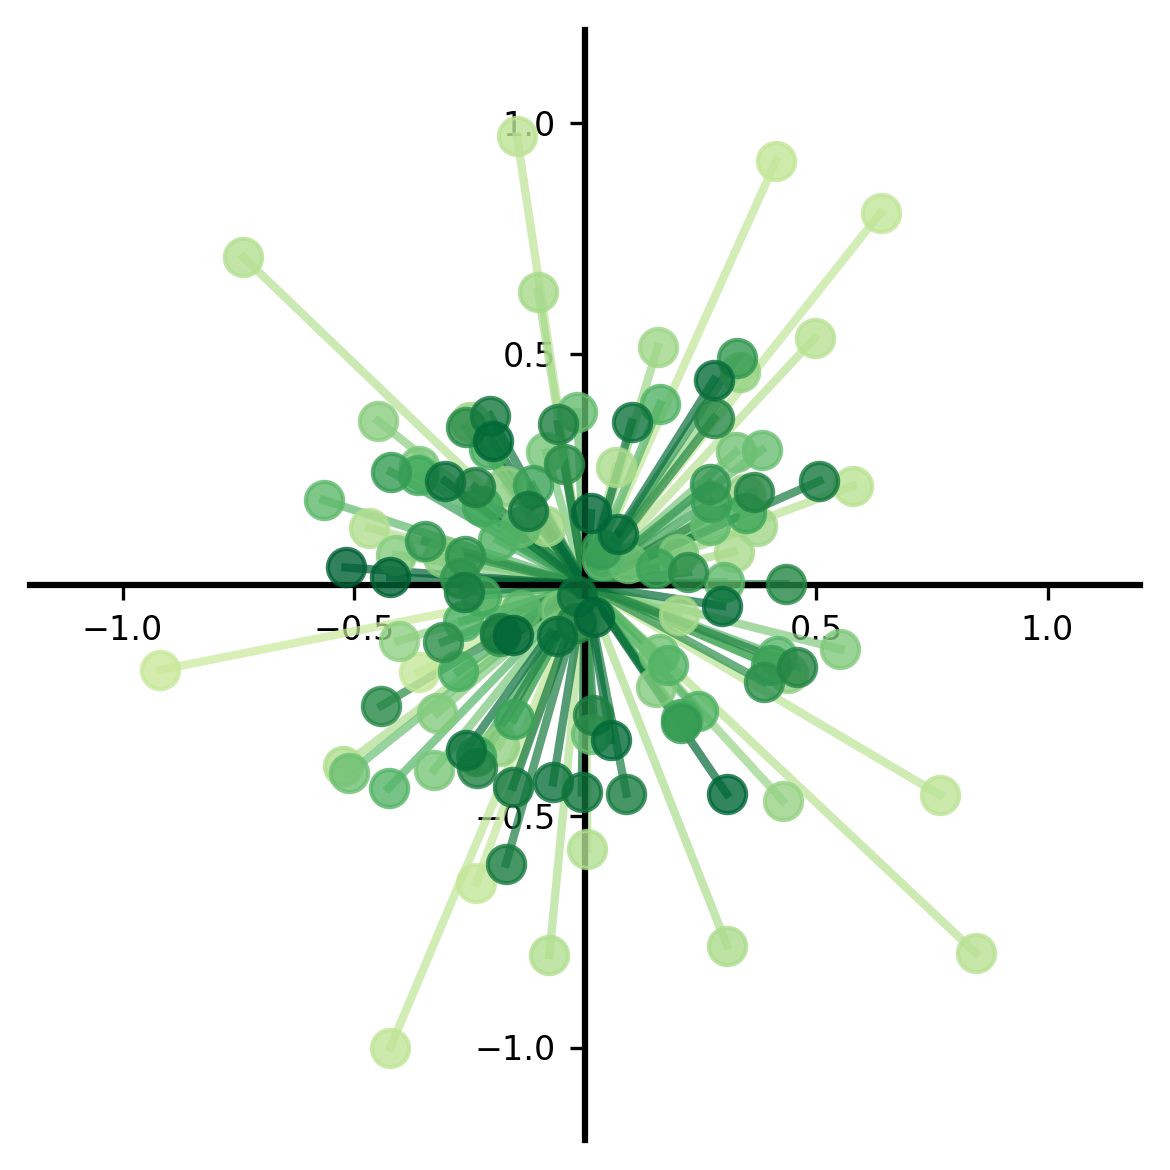
\includegraphics[width=0.45\textwidth]{figures/transformer_features.png}
    \caption{\textbf{Feature embeddings from the GPT-2-style transformer.} Each line shows one of 128 feature directions from the input projection layer, projected onto two hidden dimensions. Features exhibit approximately uniform angular spacing, the same geometric organization observed in toy autoencoders, demonstrating that the transformer distributes features to minimize pairwise interference.}
    \label{fig:transformer_features}
\end{figure}


\subsection{Translation Model Results}

The bottleneck translation model demonstrates that superposition enables practical performance under severe capacity constraints.

\paragraph{Translation quality.} Despite compressing 512-dimensional encoder outputs to just 16 dimensions, the model achieves a BLEU score of 36.34 on newsdiscussdev2015-enfr, compared to 33.8 for the baseline model without bottleneck. The bottleneck did not impair---and slightly improved---translation quality. We attribute this modest improvement to a regularization effect: the information bottleneck forces the model to discard noise and retain only the most task-relevant features, similar to the compression benefit observed in variational and information-bottleneck methods \citep{tishby2000information}.

\paragraph{Weight distribution.} The bottleneck layer weights exhibit a peaked distribution with symmetric tails, indicating the model learned structured, efficient encoding rather than random projections.

\paragraph{Embedding space visualization (Figure~\ref{fig:translation_embeddings}).} PCA visualization of the 16-dimensional bottleneck space reveals clustering of semantically related tokens. Frequent function words (articles, prepositions) occupy distinct regions from content words, suggesting the model learned to organize linguistic features efficiently despite limited capacity.

% Figure for translation embeddings
\begin{figure}[t]
    \centering
    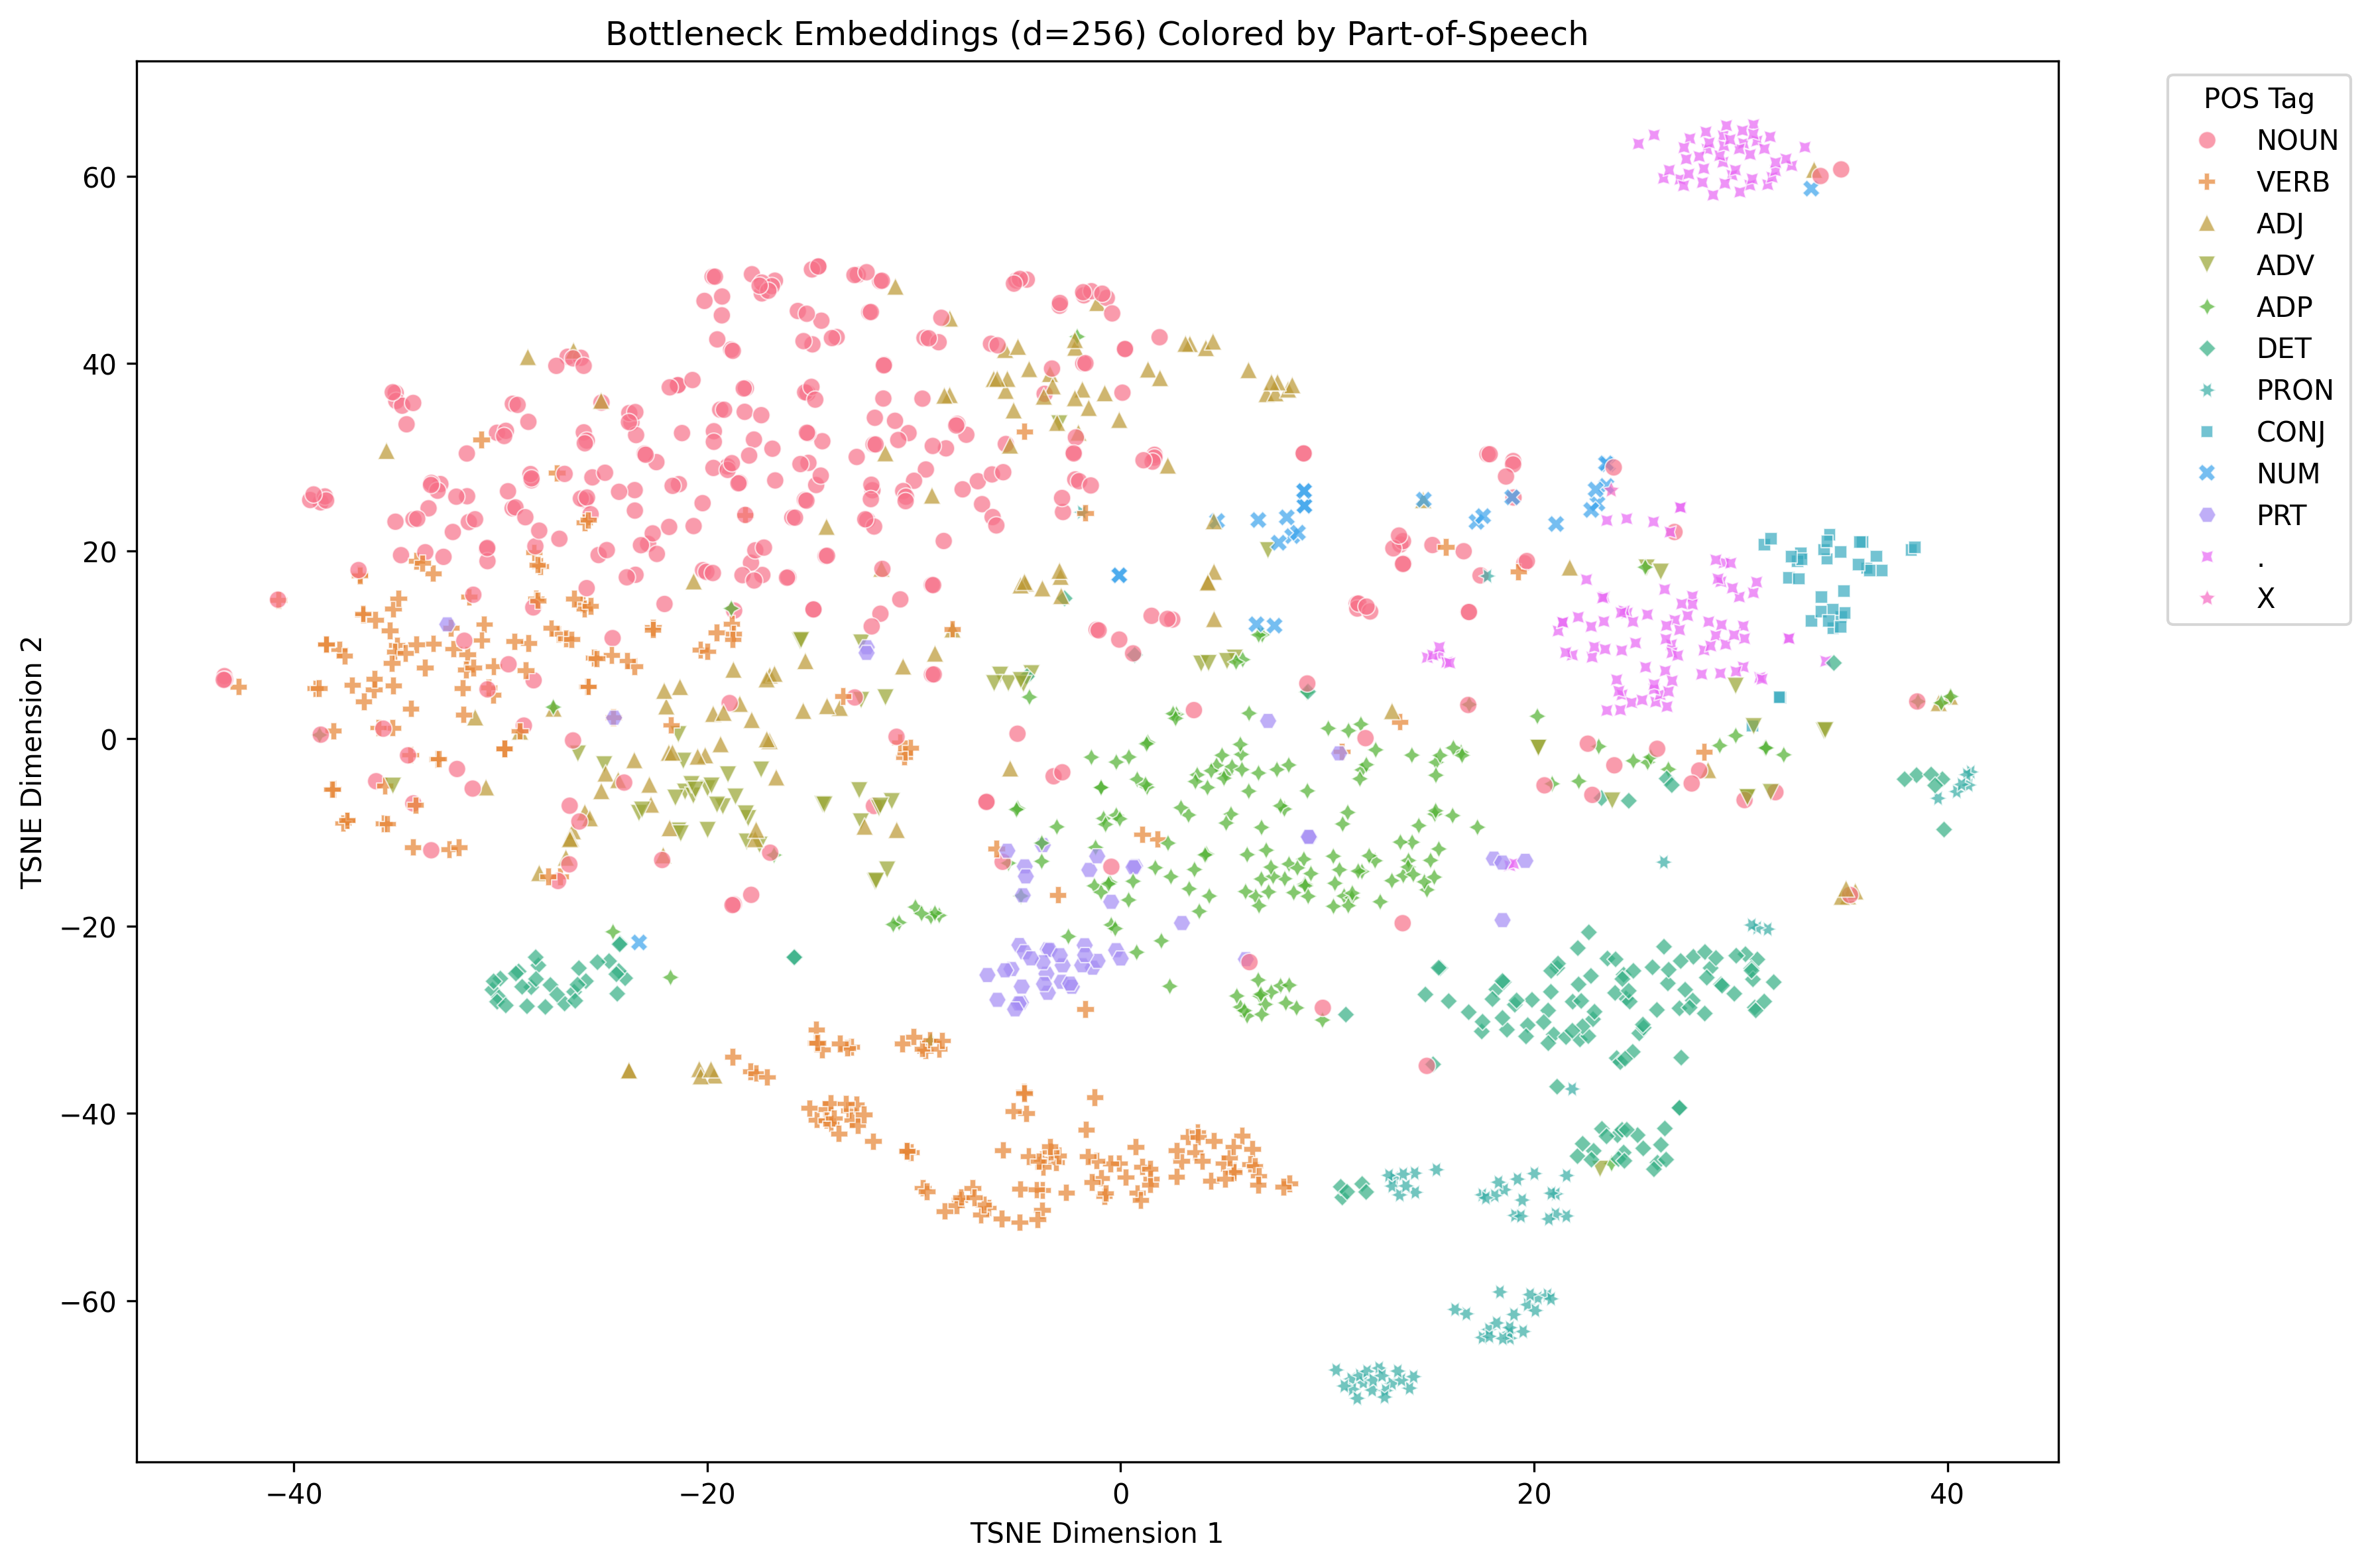
\includegraphics[width=0.8\textwidth]{images/translation_embeddings.png}
    \caption{\textbf{Embedding space of translation model bottleneck layer.} 3D PCA projection of the 16-dimensional bottleneck representations. Each point represents a token; labeled points show frequent French and English words. Semantic clustering is visible: function words (articles, prepositions) cluster separately from content words, suggesting structured encoding despite severe dimensional constraint (512$\rightarrow$16 dimensions).}
    \label{fig:translation_embeddings}
\end{figure}

\subsection{Cross-Architecture Summary}

Table~\ref{tab:full_comparison} synthesizes results across all model families, from the toy autoencoder to the full-scale Coconut model. Superposition emerges consistently whenever $n > d$, with interference structure governed by the compression ratio and architectural capacity.

\begin{table}[t]
\centering
\caption{Summary of superposition metrics across all architectures. $n$: number of features; $d$: bottleneck dimension; $n/d$: compression ratio; $\mu_{\max}$: maximum coherence; $\bar{\mu}$: mean coherence; Orth.\%: fraction of near-orthogonal pairs ($|G_{ij}| < 0.1$). Models are ordered by compression ratio.}
\label{tab:full_comparison}
\small
\begin{tabular}{llrrcccc}
\toprule
\textbf{Model} & \textbf{Type} & $n$ & $d$ & $n/d$ & $\mu_{\max}$ & $\bar{\mu}$ & \textbf{Orth.\%} \\
\midrule
Translation & Repr. & 512 & 256 & 2.0$\times$ & 0.315 & 0.055 & 85.4\% \\
Toy autoenc. & Repr. & 5 & 2 & 2.5$\times$ & 0.998 & 0.549 & 10.0\% \\
CT-$d256$ & Repr. & 768 & 256 & 3.0$\times$ & 0.404 & 0.064 & 78.7\% \\
CO-$d256$ & Reas. & 768 & 256 & 3.0$\times$ & 0.303 & 0.050 & 89.0\% \\
Computation & Repr. & 10 & 3 & 3.3$\times$ & 1.000 & 0.496 & 17.8\% \\
CT-$d128$ & Repr. & 768 & 128 & 6.0$\times$ & 0.497 & 0.088 & 63.6\% \\
CO-$d128$ & Reas. & 768 & 128 & 6.0$\times$ & 0.395 & 0.071 & 74.1\% \\
CT-$d64$ & Repr. & 768 & 64 & 12$\times$ & 0.628 & 0.116 & 50.5\% \\
CO-$d64$ & Reas. & 768 & 64 & 12$\times$ & 0.564 & 0.100 & 57.3\% \\
CT-$d32$ & Repr. & 768 & 32 & 24$\times$ & 0.776 & 0.162 & 36.9\% \\
CO-$d32$ & Reas. & 768 & 32 & 24$\times$ & 0.711 & 0.142 & 42.2\% \\
\bottomrule
\end{tabular}
\end{table}

Several patterns emerge from this comparison. First, \textbf{compression ratio governs interference}: across architectures, higher $n/d$ consistently produces higher $\mu_{\max}$ and lower orthogonal fractions, holding for both toy models and practical language models alike. Second, \textbf{Coconut outperforms CT at every $d$}. At matched compression ratios, Coconut achieves 5--14\% more orthogonal pairs and 8--20\% lower $\mu_{\max}$ than CT, an advantage attributable to the iterative reasoning mechanism (Section~\ref{sec:timespace_empirical}).

Perhaps more striking is that \textbf{large-$n$ models achieve dramatically better packing}. The translation model ($n=512$, $d=256$) achieves 85.4\% orthogonality at only 2$\times$ compression, far better than the toy model (10.0\% at 2.5$\times$). High-dimensional spaces offer exponentially more nearly-orthogonal directions, consistent with the $n_{\text{eff}} = O(d + d/\sqrt{1-S})$ scaling of Corollary~\ref{cor:capacity}. Taken together, these results demonstrate that \textbf{superposition is universal}: every model with $n > d$ exhibits non-trivial superposition, whether it is a toy autoencoder, a frozen translation model, a GPT-2 transformer, or an iterative reasoning architecture trained on natural language.

The consistent emergence of superposition across these diverse architectures raises a natural question: is superposition limited to \emph{representational} settings---packing static features into limited dimensions---or does the same phenomenon extend to \emph{reasoning}, where models maintain multiple reasoning traces in latent space? We investigate this connection in the following sections.
